\documentclass[a4paper,pdf]{article}
\usepackage{hyperref}
\usepackage{pdfpages} % http://mirror.unl.edu/ctan/macros/latex/contrib/pdfpages/pdfpages.pdf
\usepackage{booktabs} 
\begin{document}




%%% DIT IS DE TITLE PAGE VOOR INFORMATIEKUNDE NIET VOOR AI OF INFORMATICA! 
%% GEBRUIK VOOR AI OF INFORMATICA JE EIGEN TITLEPAGE TEMPLATES\


\begin{center}

\vspace{2.5cm}

% [CHANGE] The title of your thesis. If your thesis has a subtitle, then this
% should appear right below the main title, in a smaller font.
\begin{Huge}
Title of the thesis
\end{Huge}

\vspace{1.5cm}

% [CHANGE] Your full name. In case of multiple names, you can include their
% initials as well, e.g. "Jan G.J. van der Wegge".
Jan van der Wegge\\
% [CHANGE] Your student ID, as this has been assigned to you by the UvA
% administration.
9123456

\vspace{1.5cm}

% [DO NOT CHANGE]
Bachelor thesis\\
% [CHANGE] Whether your Bachelor thesis is 6 ECTS (regular) or 9 ECTS (Honours
% programme).
Credits: 12 EC

\vspace{0.5cm}

% [DO NOT CHANGE] The name of the educational programme.
Bachelor Opleiding Informatiekunde

\vspace{0.25cm}

% [DO NOT CHANGE] The addess of the educational programme.
University of Amsterdam\\
Faculty of Science\\
Science Park 904\\
1098 XH Amsterdam

\vspace{4cm}

\emph{Supervisor}\\
% [CHANGE] The name of your supervisor. Include the titles of your supervisor,
% as well as the initials for *all* of his/her first names.
Dr. M. J. Marx

\vspace{0.25cm}

% [CHANGE] The address of the institute at which your supervisor is working.
% Be sure to include (1) institute (is appropriate), (2) faculty (if
% appropriate), (3) organisation name, (4) organisation address (2 lines).
ILPS, IvI\\
Faculty of Science\\
University of Amsterdam\\
Science Park 904\\
1098 XH  Amsterdam

\vspace{1.5cm}

% [CHANGE] The date at which you will finalize and submit your thesis.
2016-06-26

\end{center}



\pagebreak

\tableofcontents

\pagebreak

\begin{abstract}
% [CHANGE] 
\end{abstract}


\pagebreak


% Here you input all your sections in seperate files

\section{Introduction}
\label{sec:intro}
\begin{itemize}
\item Bevat je onderzoeksvraag (of vragen)
\item Plaatst je vraag in de bestaande literatuur.
\end{itemize}

Je onderzoeksvraag is leidend voor je hele scriptie. Alles wat je doet moet uiteindelijk terug te voeren zijn op 1 doel: het beantwoorden van die vraag. 

Typisch zal je het dan ook zo doen:

Mijn onderzoeksvraag is onderverdeeld in de volgende deelvragen:

\begin{description}
\item[RQ1] \ldots We   beantwoorden deze vraag  door het volgende te doen/ antwoord op de volgende vragen te vinden/ \ldots
\begin{enumerate}
\item Vragen op dit niveau kan je echt beantwoorden, en dat doe je in je Evaluatie sectie~\ref{sec:eva}.
\end{enumerate}
\item[RQ2] \ldots
\item[RQ3] \ldots
\end{description}

Je Evaluatie sectie~\ref{sec:eva} bevat evenveel subsecties als je deelvragen hebt. En in elke sectie beantwoord je dan die deelvraag met behulp van de vragen op het onderste niveau.

In je conclusies kan je dan je hoofdvraag gaan beantwoorden op basis van al het eerder vergaarde bewijs.


\paragraph{Overview of thesis}
Hier geef je even kort weer wat in elke sectie staat.
\section{Related Work}
\label{sec:rel}

Deze sectie bestaat uit een aantal "blokken", waarin je per blok de relevante literatuur beschrijft. 

Neem alleen literatuur op die van belang is voor jouw onderzoeksvraag en deelvragen.

Typisch heb je 1 blok voor je hoofdvraag en per deelvraag \textbf{RQi} een blok. 


\subsection{RQ1}

\subsection{RQ2}
\section{Methodology}
\label{sec:meth}


\subsection{Description of the data}
The dataset is a set of lobby documents scraped from the web. Lobbying can be defined as the act of attempting to influence decisions made by officials in a government, most often legislators or members of regulatory agencies. Lobby documents are for example: resolutions, chamber inquiries, letters to the government and more. A distribution of different types can be seen in figure \ref{fig:data_dis}. The result of scraping these documents is that certain figures or itemization structures are textualized into words concatenated with itemization numbers, table entry titles or something similar. However, Frog's tokenization module will most of the time find the correct tokens.  These documents are exported as consistent JSON dicts, with for each doc corresponding meta information about the document such as the document ID, source, and type. The format can easily be read with Python. For domain reduction purposes, only parliamentary items are included in the data set. These items form the majority of the items and are in itself a mix of all types, except for the news items, in which the named entities vary greatly in domain compared to the Parliamentary Items.

\begin{tabular}{l*{6}{c}r}\label{fig:data-dis}
Type              & Count \\
\hline
Parliamentary item & 131906  \\
News item & 95261 \\
Chamber inquiry & 38804  \\
Voting & 20930 \\
Chamber letter & 19828
Agenda item & 18950  \\
Resolutions & 4792 \\
\end{tabular}

\subsection{Methods}
The following sections will describe the stages required to examine the suitability of Frog for doing NER on Parliamentary Items. I will first describe how Frog has been used. Then I will go over the preparation needed to evaluate Frog on the CoNLL-2002 data set and the set of Parliamentary Items. Lastly I will explain how the reclassification of entity types was performed. 

\subsubsection{Frog usage}
Frog is open-source software that can be modified or redistributed under the GNU General Public License\footnote{\url{http://www.gnu.org/copyleft/gpl.html}}. The results in this paper are acquired by running Frog through a virtual machine on Windows. All necessary dependencies of Frog, including Frog itself, are provided by the LaMachine software distribution\footnote{\url{https://proycon.github.io/LaMachine/}}. Frog can be run through Python using the python-frog binding which is also inlcuded in the virtual machine.

\subsubsection{Evaluation method}
The CoNLL-2002 data set uses the format of figure \ref{fig:conll}. Every line contains three things, each seperated by space: the token, which is an unprocessed word from a sentence, the token its corresponding part-of-speech, and the token its IOB-tag. Frog its Folia output looks similar with tab-delimited column format , but with additional information per token. To release Frog on CoNLL, the test set first has to be reformatted to its original text. This is done by removing the PoS and IOB-tags, concatenating the remaining words into their original sentences thereafter.  Frog chunks together multi-word entities and other words that are closely related on one line in the output. This will make it differ from the CoNLL output, as such the output is splitted with python using regular expressions. Now the processed text has the same line mapping per token as CoNLL.

It needs to be taken into account that the annotation guidelines for the SoNar corpus differ from CoNLL. SoNar has a wider range of entity types, such as EVE for event and PRO for product. These types are annotated in CoNLL as MISC. Therefore the additional types that Frog outputs are mapped to MISC. There is also a guideline difference regarding locational adjectives, such as 'Dutch' or 'European'. CoNLL guidelines annotate such an adjective as MISC, while Frog is trained to assign LOC as type. These LOC outputs of Frog have to be reassigned to MISC as well.

\subsubsection{Reclassification of entity types}
In the case of unknown words the contextual word relations may indicate a type correctly, however, with multiple occurrences of the same unambiguous entity throughout a text, context differs from time to time. As a result an entity can be tagged correctly as a PER 90% of the time, but have an incorrect type assigned for the remaining 10%. This is expected to be resolved using \textbf{majority voting}. In the case when a certain type is dominant over a minority, this minority is reclassified as the dominant type. To retrieve information regarding the dominant types per entity, a train set of thousand parliamentary items has been processed by Frog. The total occurrences of the entity types have been counted over all documents. For each token in the test set that has been assigned to be an entity, we perform majority voting. Whether an entity type is dominant for that entity is decided based on a threshold value. When the fraction of an entity type over the total amount of entity type counts is larger than the threshold value, the type is considered dominant.

Secondly, Frog's entity type knowledge is enriched by feeding it a gazetteer in the domain of parliamentary items. This gazetteer is constructed with a combination of automatic extraction of entities with Frog and manual annotation of the correct type. The automatic extraction is performed on the training set of thousand parliamentary items. The extracted entities are sorted on popularity, giving annotation  priority to the most common entities.



\section{Evaluation}
\label{sec:eva}

Met een subsectie voor elke deelvraag.

In hoeverre is je vraag beantwoord?

Een mooie graphic/visualisatie is hier heel gewenst.

Hou het kort maar krachtig.
\section{Conclusions}
\label{sec:conc}
The high recall in the evaluation results indicates that Frog is very capable in retrieving all relevant entities in a text. Type assignment, however, has appeared to be substantually more difficult. As a solution, reclassification of entity types has been proposed, and has proven to  increase overall type-precision. The semi-automatic construction of a parliamentary gazetteer as auxilliary, makes Frog well suitable for the NER-task required for the suggested system. Since a semi-automatic gazetteer can be constructed for any given domain, in addition to the fact that majority voting is domain-independent, Frog can be exported to similar Dutch NER-tasks.

\section{Discussion of approach}


\section{Acknowledgements}
%TODO
%Hier kan je bedanken wie je maar wilt.

% your refs

\bibliographystyle{plain}
\bibliography{MyThesis}

\appendix

%\section{Suggested system} \label{app:sug_sys}
\subsection{System overview}
The system in mind requires three variable inputs:
\begin{enumerate}
\item The dump file obtained after running Frog with all NE's per item
\item The original data file with the documents (because the source isn't included in the dump file)
\item The search query
\end{enumerate}
A user of the system has two options: either acquire the NE's in a selected document (without necessary prior knowledge of its contents), or find a document that is most relevant to the search query of the user. The query has to be of the following format: $$TYPE{\text{:}}NE(+TYPE{\text{:}}NE)^n$$ An NE can be negated by putting a '!' right before the term. The result of running the code below using the default parameters can be seen in figure \ref{fig:sys_out}.

\subsubsection{Alternating the search query}\label{app:alt_query}
If the company \textit{Coca-Cola} is not classified as ORG, but as a MISC instead, the following search query will not retrieve results: $$ORG\text{:}Coca\text{-}Cola$$
However, adding another possible type to the query fixes the issue:
$$ORG\text{:}Coca\text{-}Cola\text{+}MISC\text{:}Coca\text{-}Cola$$
In contrast, when \textit{Coca-Cola} is not \emph{recalled}, there is no alternate query that will retrieve the NE. 

\begin{figure}
    \centering
    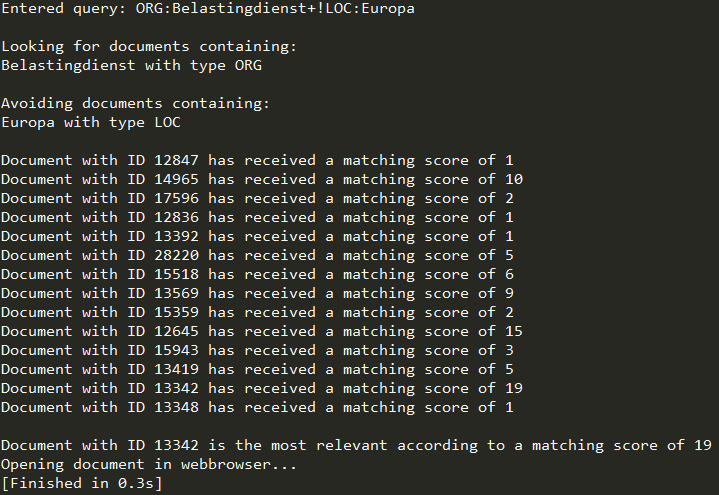
\includegraphics[scale=0.8]{fig/sys_out}
    \caption{The command line output running the code of the suggested system}
    \label{fig:sys_out}
\end{figure}

\subsection{Raw code}
\begin{lstlisting}
import json, re, webbrowser, sys, argparse
from operator import itemgetter

def main(dump_path, docs_path, query):
    with open(dump_path) as f:
        dump = json.load(f)

    winning_id = get_document(query, dump)

    with open(docs_path) as g:
        for doc in g:
            doc = json.loads(doc)
            if winning_id == doc['_id']:
                print 'Opening document in webbrowser...'
                webbrowser.open(doc['_source']['url'])    

def get_document(query, dump):
    """
    Opens the document most relevant
    to the query in your webbrowser from its 
    original source.
    """
    relevant_docs = []
    positive = []
    negative = []
    elements = query.split('+')

    print 'Entered query:', query

    ## Seperate the query into a list of wanted and unwanted entities in a doc
    for e in elements:
        entity_type, entity = e.split(':')
        if entity_type[0] == '!':
            negative.append((re.sub('!', '', entity_type), entity))
        else:
            positive.append((entity_type, entity))

    print '\n', 'Looking for documents containing:'
    for entry in positive:
        print entry[1], 'with type', entry[0]

    print '\n', 'Avoiding documents containing:'
    for entry in negative:
        print entry[1], 'with type', entry[0]

    for doc_id in dump:
        if matches_query(dump[doc_id], positive, negative):
            relevant_docs.append(doc_id)

    return most_relevant_doc_id(relevant_docs, query, dump)

def matches_query(doc, positive, negative):
    """
    Returns if the document matches the query
    by checking wanted and unwanted entities
    """
    match = False

    ## Look for a positive match
    for entity_type, entity in positive:
        if entity in doc['entities']:
            for tag in doc['entities'][entity]:
                t = tag.split('-')[1]
                if t == entity_type:
                    match = True
    
    ## If positive, look for a negative match
    if match:
        for entity_type, entity in negative:
            if entity in doc['entities']:
                for tag in doc['entities'][entity]:
                    t = tag.split('-')[1]
                    if t == entity_type:
                        match = False

    return match


def most_relevant_doc_id(relevant_docs, query, dump):
    """
    Returns the document ID with the highest
    matching score.
    """
    matching_scores = []
    for doc in relevant_docs:
        score = calculate_matching_score(dump[doc], query)
        matching_scores.append((doc, score))

    print ''
    for pair in matching_scores:
        print 'Document with ID %d has received a matching score of %d'%(int(pair[0]), pair[1])


    ID, best_score = max(matching_scores, key=itemgetter(1))
    print '\n', 'Document with ID %d is the most relevant according to a matching score of %d'%(int(ID), int(best_score)) 

    return ID
        

def calculate_matching_score(doc, query):
    """
    Returns the document's matching score
    to the query
    """ 
    elements = query.split('+')
    positive = []
    score = 0

    ## Get all wanted entities and their type out of the query
    for e in elements:
        entity_type, entity = e.split(':')
        if not entity_type[0] == '!':
            positive.append((entity_type, entity))

    ## Look for a positive match, and increase matching score accordingly
    for entity_type, entity in positive:
        if entity in doc['entities']:
            for tag in doc['entities'][entity]:
                t = tag.split('-')[1]
                if t == entity_type:
                    score += doc['entities'][entity][tag]

    return score

if __name__ == '__main__':

    p = argparse.ArgumentParser()
    p.add_argument('-dump', type=str, help='path to the dump with extracted entities per doc', default='data/lobby/dump')
    p.add_argument('-docs', type=str, help='path to original unprocessed documents', default='data/lobby/train_documents')
    p.add_argument('-query', type=str, help='Query used to find the desired document', default='ORG:Belastingdienst+!LOC:Europa')
    args = p.parse_args(sys.argv[1:])

    main(args.dump, args.docs, args.query)



 
\end{lstlisting}


\section{Slides}

% Example
\includepdf[nup=2x3 , pages=-]{sargent-lecture_slides.pdf}
 
\end{document}
